\chapter{Background} \label{chap2}
\renewcommand{\headrulewidth}{0pt}
\lhead[\thepage]{\leftmark}
\rhead[\leftmark]{\thepage}
\cfoot[]{}

\section{Air pollution}
\subsection{Introduction}

Air pollution stands as a critical environmental issue, significantly impacting human health, ecosystems, and climate patterns. According to the World Health Organization (WHO) in 2020, approximately seven million deaths worldwide were attributed to air pollution \citep{who2020world}. Air pollutants such as nitrogen oxides (NO\textsubscript{x} = NO + NO\textsubscript{2}), carbon monoxide (CO), ground-level ozone (O\textsubscript{3}), sulfur dioxide (SO\textsubscript{2}) and particulate matter (PM), are directly emitted from natural or anthropogenic activities or through atmospheric photochemical reactions. Some pollutants are emitted alongside carbon dioxide (CO\textsubscript{2}) during combustion processes, while others act as short-lived climate forcers, directly or indirectly influencing climate change by affecting the global radiation budget \citep{RN3}. Moreover, ozone can negatively affect crop yield, presenting potential challenges to future food security \citep{avnery2011global, avnery2011global2, chuwah2015global, tai2017impacts}. \par
Nitrogen dioxide (NO\textsubscript{2}) is a particularly worrisome pollutant due to its adverse effects on human health \citep{hamra2015lung}. Short-term exposure to elevated NO\textsubscript{2} concentrations can induce airway inflammation, increase susceptibility to respiratory infections and allergies, and worsen pre-existing lung or heart conditions \citep{bono2016air, kelly2011air}. Furthermore, NO\textsubscript{x} induces environmental changes by altering soil chemistry and biodiversity through nitrogen deposition via dry and wet processes \citep{bobbink2010global}. Additionally, NO\textsubscript{x} plays a crucial role as a precursor to tropospheric ozone (O\textsubscript{3}), alongside volatile organic compounds (VOCs) \citep{akimoto2022rethinking}. NO\textsubscript{x}, CO, and non-methane volatile organic compounds (NMVOCs) influence the lifetime of methane (CH\textsubscript{4}) by affecting the atmospheric mixing ratio of hydroxyl radicals (OH) \citep{akimoto2022rethinking}, which serve as a primary sink for CH\textsubscript{4} \citep{turner2019interpreting}. Both O\textsubscript{3} and CH\textsubscript{4} are short-lived climate pollutants (SLCPs) that contribute to positive radiative forcing, thereby exacerbating global warming \citep{akimoto2022rethinking}. \par

Global NO\textsubscript{x} emissions primarily result from fossil fuel combustion in the energy, industry, and transportation sectors. In 2017, the energy generation (22\%), industry (15\%), and on-road transportation (23\%) sectors collectively accounted for nearly 60\% of global NO\textsubscript{x} emissions. Notably, these sectors significantly contributed to emissions from coal combustion, with the energy and industry sectors alone contributing over 46\% of the total emissions. Furthermore, the combined combustion of liquid fuels (oil) and natural gas constituted 100\% of on-road NO\textsubscript{x} emissions \citep{mcduffie2020global}. Examining historical emissions from 1970 to 2017 documented in the CEDS database \citep{mcduffie2020global}, global NO\textsubscript{x} emissions peaked between 2011 and 2013, followed by a subsequent 7\% decrease by 2017. This decline was primarily attributed to more stringent emission standards implemented in North America and Europe since 1992 and in China since 2013 \citep{mcduffie2020global, zheng2018trends}. Nevertheless, within the same timeframe, global NO\textsubscript{x} emissions from the energy and industry sectors experienced a substantial increase, nearly multiplying six-fold between 1970 and 2011. This upsurge was predominantly fueled by regional increments in China, India, the Other Asia/Pacific region, and several African countries. The subsequent reduction in emissions between 2011 and 2017 was mainly a result of stringent emission control policies in China, specifically aimed at coal-fired power plants and industrial coal use \citep{zheng2018trends, liu2015reduced}. \par


In Japan, measures have been in place since the 1950s to control air pollutant emissions from various stationary and mobile sources \citep{ito202130}. An analysis of air pollution trends in Japan from 1970 to 2018 \citep{ito202130, kannari2013thirty, wakamatsu2013air} demonstrates a consistent decline in the concentrations of PM\textsubscript{2.5}, NO\textsubscript{2}, and SO\textsubscript{2}, indicating the direct effectiveness of human-induced emission control strategies in mitigating pollution levels. The decline in pollutant concentrations corresponds with specific measures taken to address emissions. For instance, the decrease in NO\textsubscript{x} levels may be attributed to the implementation of more stringent regulations governing vehicle emissions. Likewise, the decrease in SO\textsubscript{2} levels may be associated with the widespread adoption of marine fuels with lower sulfur content, highlighting the direct impact of focused interventions on reducing pollution. However, there has been a persistent year-on-year rise in ozone concentrations across broad areas in Japan, including rural zones unaffected by direct anthropogenic sources of air pollutants \citep{ito202130}. \par

\subsection{Impact of weather variations on air pollution changes}

Air pollution levels are influenced not only by emissions themselves but also by meteorological conditions. The lifetime of NO\textsubscript{2} is strongly influenced by meteorological parameters and photochemical reactions \citep{barre2021estimating} and varies seasonally \citep{dragomir2015modeling,kendrick2015diurnal}. During winter, photochemical reaction activity is reduced, resulting in a longer lifetime of the NO\textsubscript{2}. Additionally, seasonal variations in NO\textsubscript{2} concentration are controlled by dispersion processes which are significantly affected by changes in boundary layer height (BLH), wind speed and direction patterns due to temperature inversions in summer and winter \citep{barre2021estimating,kendrick2015diurnal}. Changes in seasonal meteorological patterns, such as temperature and radiation, have also been documented as factors influencing local variations in ozone in China \citep{yang2019study, yu2021review}. \par

Earlier research underscored the substantial impact of meteorological fluctuations on ozone levels in Japan. Specifically, \citep{kurokawa2009influence} emphasized the sensitivity of springtime ozone variation in Japan to outflows from continental Asia. They identified a correlation between springtime ozone and the El Niño-Southern Oscillation, suggesting a relationship where higher and lower springtime ozone levels are associated with La Niña and El Niño, respectively. The summer of 2019 saw widespread instances of elevated ozone concentrations across Japan, as reported by \citep{fukunaga2021relationship, ito202130}. According to \citep{fukunaga2021relationship}, the favorable conditions for increased ozone levels during this period were linked to clear skies and higher temperatures. They proposed that a migrating anticyclone might have transported ozone and its precursors eastward, contributing to this phenomenon. This underscores the significance of not only examining the direct impact of air pollution control measures but also understanding the role of meteorological conditions in shaping air pollution dynamics. Investigating these interdependencies could significantly improve our ability to formulate more effective measures for mitigating air pollution. \par

\section{Greenhouse gas}
\subsection{Fossil fuel GHGs}

GHGs are atmospheric gases that trap heat and contribute to warming the Earth. The major ones include carbon dioxide (CO\textsubscript{2}), methane (CH\textsubscript{4}), nitrous oxide (N\textsubscript{2}O) and Fluorinated gases (F-gases) like hydrofluorocarbons (HFCs), perfluorocarbons (PFCs), and sulfur hexafluoride (SF\textsubscript{6}). These gases persist in the atmosphere for various durations, ranging from a few years to thousands of years. They reach a well-mixed state, meaning their concentrations worldwide remain relatively consistent regardless of their sources. 
These gases differ significantly in their impact on atmospheric warming. \par
GHGs originate from diverse sources, encompassing both natural processes and human activities. Carbon dioxide is naturally present in the atmosphere as part of the Earth's carbon cycle, which is consistently exchanged carbon among the atmosphere, oceans, soil, plants, and animals. Human activities are altering the carbon cycle–both by adding more carbon dioxide to the atmosphere and by influencing the ability of natural sinks, like forests and soils, to remove and store carbon dioxide from the atmosphere. While carbon dioxide emissions originate from various natural sources, human-induced emissions have been primarily responsible for the substantial increase in GHGs in the atmosphere since the Industrial Revolution commenced around 1750 \citep{RN3}. In 2019, emissions included approximately 45 ± 5.5 GtCO\textsubscript{2} emissions, 11 ± 3.2 GtCO\textsubscript{2}-eq of methane (CH\textsubscript{4}), 2.7 ± 1.6 GtCO\textsubscript{2}-eq of nitrous oxide (N\textsubscript{2}O) and 1.4 ± 0.41 GtCO\textsubscript{2}-eq of fluorinated gases (F-gases) \citep{keylist}. The primary source of carbon dioxide stems from the combustion of fossil fuels within energy conversion systems like boilers in electric power plants, engines in aircraft and automobiles, and in cooking and heating within homes and businesses, accounting for approximately 64\% of emissions. Fossil fuels also play a significant role in methane emissions, the second-largest contributor to global warming. While most GHGs originate from fossil fuel combustion, about one quarter comes from land-related activities like agriculture (mainly methane and nitrous oxide) and deforestation (mainly carbon dioxide). Additional emissions come from industrial processes (primarily carbon dioxide, nitrous oxide, and F-gases), as well as municipal waste and wastewater (mainly CH\textsubscript{4}) \citep{keylist}. 
The estimated global net anthropogenic GHGs emissions for the year 2019 reached approximately 59 ± 6.6 GtCO\textsubscript{2}-eq, marking a 12\% increase compared to the levels seen in 2010 and a significant 54\% surge compared to the figures from 1990. Among these emissions, the dominant share and escalating growth came from CO\textsubscript{2} emissions originating from fossil fuels combustion and industrial processes (CO\textsubscript{2}-FFI), followed closely by methane emissions. Notably, the highest relative growth occurred in F-gases, albeit starting from minimal levels in 1990. During 2010–2019 period, the average annual GHG emissions surpassed those of any preceding decade on record. However, the rate of growth between 2010 and 2019 (1.3\% yr\textsuperscript{-1}) was comparatively lower than that observed between 2000 and 2009 (2.1\% yr\textsuperscript{-1}). In 2019, a substantial 79\% of global GHGs emissions stemmed from energy, industry, transport, and building sectors combined, while 22\% originated from agriculture, forestry, and other land use (AFOLU). Global gross domestic product (GDP) per capita and population growth remained the primary drivers of CO\textsubscript{2} emissions from fossil fuel combustion throughout the last decade. The trends from 1990 continued through the years 2010-2019, with GDP per capita and population growth contributing to emissions escalation by 2.3\% yr\textsuperscript{-1} and 1.2\% yr\textsuperscript{-1}, respectively. This growth outpaced the reduction in the use of energy per unit of GDP (-2\% yr\textsuperscript{-1}, globally) as well as improvements in the carbon intensity of energy (-0.3\% yr\textsuperscript{-1}). Therefore, emissions reductions in CO\textsubscript{2}-FFI due to improvements in energy intensity of GDP and carbon intensity of energy, have been less than emissions increase from rising global activity levels in industry, energy supply, transport, agriculture and buildings \citep{portner2022ipcc}. \par

\subsection{Terrestrial carbon fluxes}

Terrestrial ecosystems play a crucial role in mitigating global warming by serving as a persistent carbon sink, actively absorbing and storing excess carbon dioxide from the atmosphere \citep{pan2011large}. Over the period from 2010 to 2019, the terrestrial CO\textsubscript{2} sink is estimated to offset fossil CO\textsubscript{2} emissions by 35\%, surpassing the ocean, which is projected to remove 26\% of fossil-fuel-derived CO\textsubscript{2} \citep{friedlingstein2020global, wang2022disentangling}. The substantial global carbon flux, known as terrestrial gross primary production (GPP), significantly contributes to the reduction of anthropogenic CO\textsubscript{2} emissions \citep{beer2010terrestrial}. \par

\begin{figure}
    \centering
    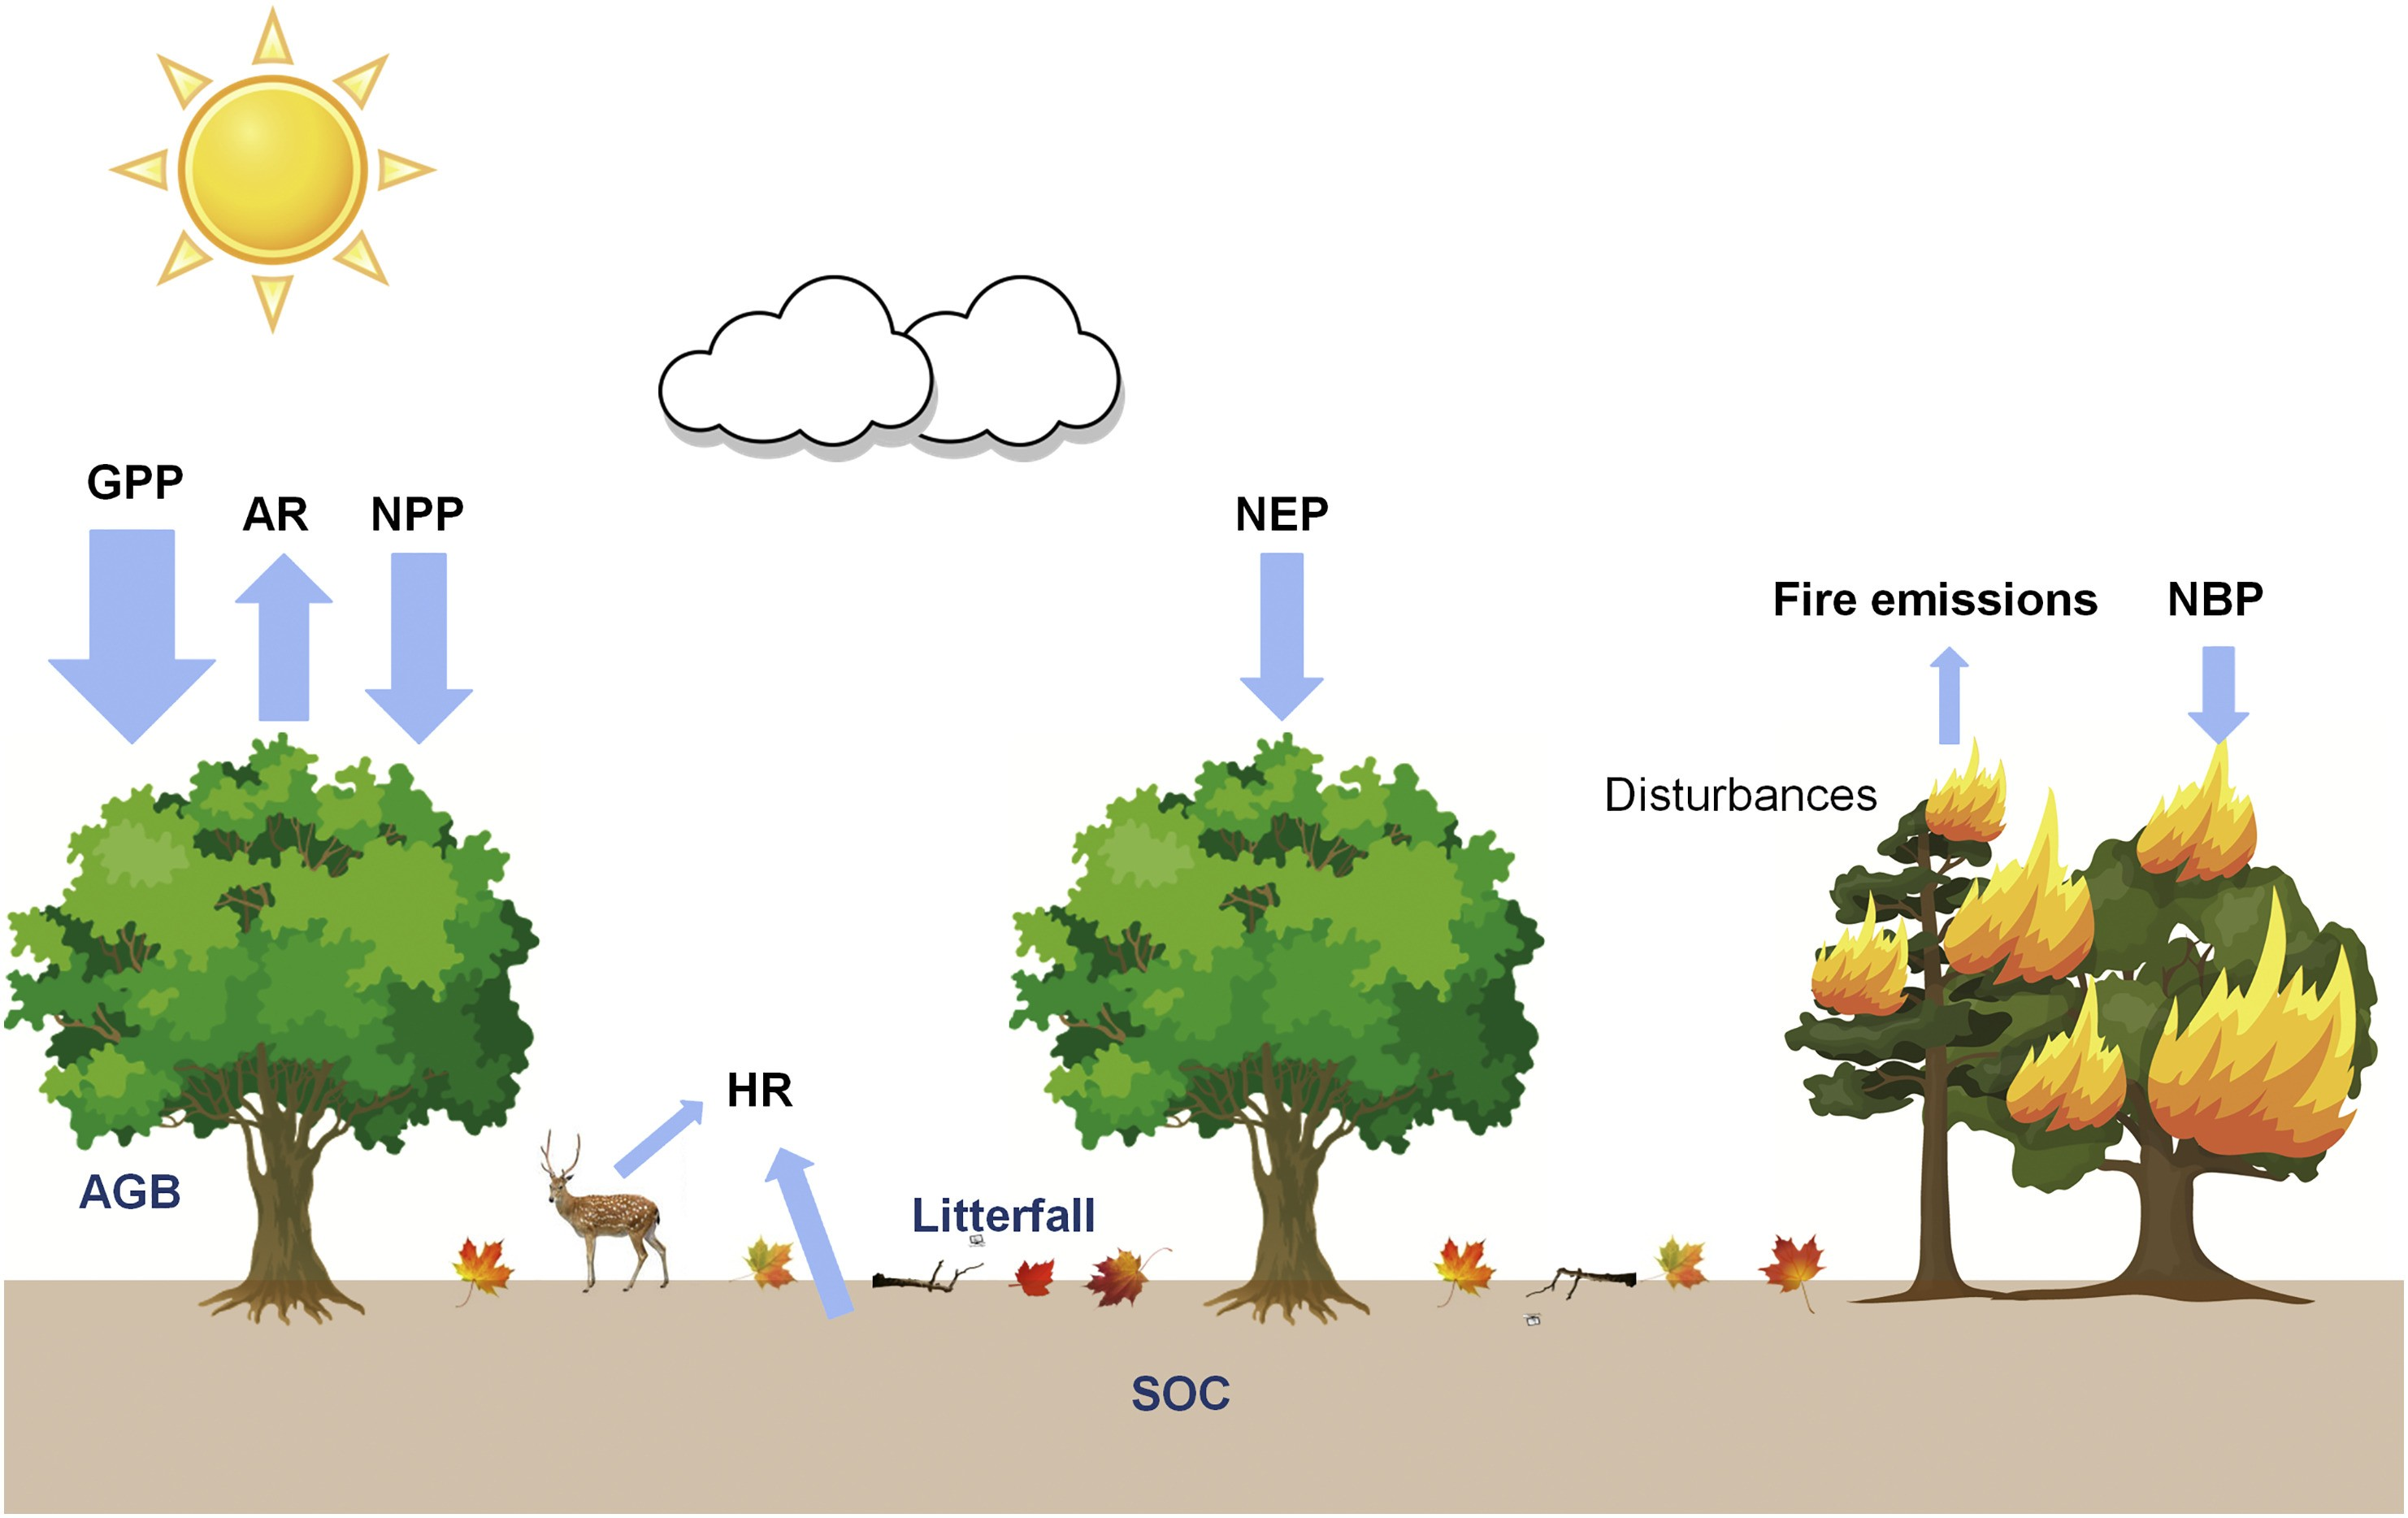
\includegraphics[width=\textwidth]{figs/chap2/fig1.jpg}
    \caption{Terrestrial carbon cycle \citep{xiao2019remote}}
    \label{fig:chap2_fig1}
\end{figure}

% need recheck
As presented in Figure \ref{fig:chap2_fig1}, we illustrate that GPP represents the total carbon sequestered by terrestrial ecosystems, serving as the foundation for food, wood, and fiber production and thereby holding significant implications for human well-being \citep{xiao2019remote}. A portion of the absorbed carbon is released back into the atmosphere through plant autotrophic respiration (AR). The disparity between GPP and AR is Net Primary Production (NPP). Soil organic carbon (SOC) accumulates from plant materials, such as leaves and branches, that fall to the ground, also known as litterfall. The size of the SOC pool is impacted by carbon inputs from litterfall and root mortality/exudation, as well as carbon release from decomposition, referred to as heterotrophic respiration (HR) \citep{liu2011simulating}. AR and HR collectively constitute ecosystem respiration (RECO). Net Ecosystem Production (NEP) is the difference between GPP and RECO. \par
Processes like deforestation, harvesting, and fires can result in carbon loss, with the net ecosystem carbon balance referred to as Net Biome Production (NBP). Disturbances, crucial ecosystem processes, impact carbon cycle dynamics. Wildfires, for example, lead to immediate carbon transfer from ecosystems to the atmosphere. Fires, along with other disturbances such as insect and disease outbreaks, droughts, severe storms, and harvesting, can cause substantial effects on GPP and respiration, with these impacts persisting for decades as ecosystems recover \citep{xiao2019remote}. \par

Estimating GPP involves various methods, such as simulating DGVMs like those employed in the TRENDY project \citep{sitch2015recent, le2018global}, upscaling from measurements obtained through eddy covariance (EC) flux tower and satellite observations \citep{jung2019fluxcom, zeng2020global}. However, all these approaches rely on plant functional types (PFTs) to estimate ecosystem productivity \citep{poulter2011plant, poulter2015plant, lin2021improved, guo2023estimating, yan2023integrating}. Inconsistencies in PFT maps can significantly contribute to uncertainties in GPP estimations, as well as other climate-relevant variables, at both regional and global scales \citep{poulter2011plant}. Particularly in the tropical region, the sparse distribution of EC sites, the high species richness of trees, and the complex vertical structure of tropical rainforests pose challenges \citep{montgomery2001forest}, making it difficult to accurately quantify the seasonality of carbon fluxes \citep{xu2015satellite}. \par

\section{Relationship between air pollution and greenhouse gas}
CO\textsubscript{2} is considered one of the most important GHGs, which has played a significant role in the current and future global climate change. Meanwhile, NO\textsubscript{2} emerges as a particularly concerning pollutant due to its adverse effects on human health and ecosystem. Their atmospheric concentration has considerably increased since the Industrial Revolution and is attributed mostly to anthropogenic sources, especially fossil-fuel combustion. While CO\textsubscript{2} emission reduction has become a goal of international agreements such as the Kyoto Protocol \citep{protocol1997united} and the Paris Agreement on Climate Change (\url{https://unfccc.int/process-and-meetings/the-paris-agreement}), the air pollution control measures reducing NO\textsubscript{2} emission have been implemented in Northern America, Europe and China to improve local air quality. Therefore, accurate knowledge of fossil fuel CO\textsubscript{2} and NO\textsubscript{2} emissions as well as their trends pose an importance both for climate prediction and mitigation policy purposes. \par

Fossil fuel combustion is mainly contributor of CO\textsubscript{2} and co-emitter NO\textsubscript{2} emission. These emissions are driven by activity such as fuel consumption, but differ by their relative proportion (i.e., emission factor)\citep{miyazaki2023predictability}. Global fossil fuel CO\textsubscript{2} emission inventories (e.g. CDIAC \citep{andres2012synthesis}, ODIAC \citep{oda2011very, oda2018open}, EDGAR \citep{crippa2020high}, FFDAS \citep{asefi2014multiyear}, and CEDS \citep{hoesly2018historical}) are compiled from available national emission inventory. Fossil CO\textsubscript{2} emissions are estimated by combining economic activity data and emissions factors, with different levels of methodological complexity (tiers) or approaches (e.g., IPCC Guidelines for National Greenhouse Gas Inventories). Several organizations or groups provide estimates of fossil CO\textsubscript{2} emissions, with each dataset having slightly different system boundaries, methods, activity data, and emissions factors \citep{andrew2020comparison}. This “bottom-up” approach based on available statistical information regarding economic activities and corresponding technologies. Such error and bias information can cause the an uncertainty that is generally within ±10\% among these inventories at global scale, however, the uncertainty in emission estimates significantly varied in different countries, from 10\% in developed countries \citep{essd-11-1783-2019} but larger uncertainty in rapidly developing countries such as 8\% to 24\% for China \citep{han2020evaluating, marland2008uncertainties} to more than 50\% for least developed countries \citep{andres2016gridded, essd-11-1783-2019, oda2018open}. For the case in China, large variations between nine emission inventories were largely due to the different emission factors related to coal quality and activity data \citep{han2020evaluating,miyazaki2023predictability}. Variations in these approaches, combined with errors in spatial allocation utilizing remote sensing source, can result in significant discrepancies in local estimates for a city or municipality \citep{oda2019errors, hutchins2017comparison}. Furthermore, these emissions data are mostly self-reported by national governments, which can take several years to produce \citep{marland2008uncertainties}. Air quality emission inventories, like fossil fuel CO\textsubscript{2} emission, use similar methods to determine fuel consumption and sector-based emission factors, and consequently incur substantial latency in their reporting \citep{miyazaki2023predictability}.\par

Recently, the "top-down" method has emerged as an additional approach for estimating fossil fuel CO\textsubscript{2} emissions, driven by advancements in satellite observations and data assimilation frameworks. This method utilizes direct CO\textsubscript{2} observations obtained from satellite imagery to estimate CO\textsubscript{2} emissions. However, existing satellites, such as the Greenhouse gases Observing SATellite (GOSAT) and Orbiting Carbon Observatory-2 (OCO-2), were designed to focus on the spatiotemporal distribution of natural carbon fluxes on regional scales rather than to quantify anthropogenic emissions \citep{nassar2017quantifying, yang2023using}. Consequently, the limitations in the spatial and temporal resolution of these CO\textsubscript{2} observations hinder their capacity to estimate CO\textsubscript{2} emissions at urban or city levels. \par

\begin{figure}[tbh!]
    \centering
    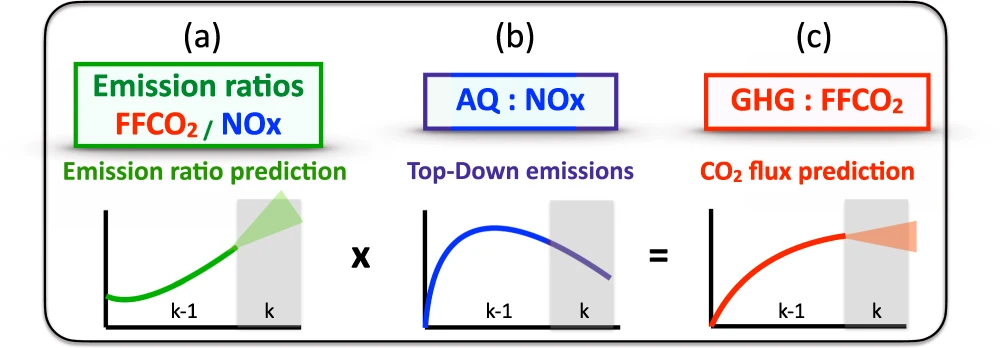
\includegraphics[width=\textwidth]{figs/chap2/aq_nox_ratio.png}
    \caption[Fossil fuel CO\textsubscript{2} prediction from top-down NO\textsubscript{x}]{Changes in CO\textsubscript{2}/NO\textsubscript{x} emission ratio for the past (t=k-1) are estimated using top-down NO\textsubscript{x} emissions and bottom-up fossil fuel CO\textsubscript{2} (FFCO\textsubscript{2}) inventories (a and b). The recent (t=k) CO\textsubscript{2}/NO\textsubscript{x} level is predicted using timeseries forecasting model based on data in the past (t=k-1) to predict (c) the CO\textsubscript{2} at the recent time (t=k) \citep{miyazaki2023predictability}.}
    \label{fig:chap2_fig2}
\end{figure}

In contrast, currently available satellite-derived NO\textsubscript{2} observations, like OMI or TROPOMI, demonstrate more advanced capabilities with higher resolutions in spatiotemporal aspects. They have the potential to function as instruments in deducing fossil fuel CO\textsubscript{2} emissions at the local level. Hence, an indirect "top-down" approach utilizes proxies such as NO\textsubscript{2} observations, leveraging their co-emission with fossil fuel CO\textsubscript{2} combustion. This indirect method proves advantageous in predicting fossil fuel CO\textsubscript{2} emissions, monitoring their temporal fluctuations while distinguishing them from biogenic sources of CO\textsubscript{2} emissions itself \citep{ciais2014current, goldberg2019exploiting}. Satellite-based NO\textsubscript{2} observations, combined with NO\textsubscript{x}:CO\textsubscript{2} inventory ratios, have been instrumental in estimating CO\textsubscript{2} emissions indirectly (see Figure \ref{fig:chap2_fig2}). These approaches have been applied at national scales in countries such as the US, Europe, China, and India \citep{konovalov2016estimation, zheng2020satellite, miyazaki2023predictability} and at city levels, such as in Wuhan \citep{zhang2023quantifying} Buenos Aires, Melbourne, and Mexico City \citep{yang2023using}. However, such analyses have not yet been conducted either at the national or municipal levels in Japan. Conducting studies employing these methodologies both at national and cities levels in Japan could provide supplemental independent datasets. These datasets would serve to refine and evaluate "bottom-up" inventories and to assess the efficacy of current climate change mitigation strategies related to reducing fossil fuel CO\textsubscript{2} emissions, contributing insights from local to global scales. Therefore, such investigations are necessary and could offer valuable information to refine our understanding of CO\textsubscript{2} emissions and strategies for mitigating climate change. \par

\section{Air pollution, GHGs and SDGs}
\subsection{Air pollution and SDGs}
While air pollution is intricately linked to almost all other SDGs, encompassing areas such as health, water, energy, economic growth, employment, infrastructure, cities, sustainable consumption and production, climate, water, and land, its significance is not clearly emphasized in the structure of the SDGs, as noted by \citep{elder2016strengthening}. To be specific, air pollution is explicitly addressed in three goals, with one target assigned to each:
\begin{itemize}
    \item \textbf{3.9 (Health)}: By 2030, substantially reduce the number of deaths and illnesses from hazardous chemicals andair, water and soil pollution and contamination.
    \item \textbf{11.6 (Cities)}: By 2030, reduce the adverse per capita environmental impact of cities, including by payingspecial attention to air quality and municipal and other waste Management.
    \item \textbf{12.4 (Responsible consumption and production)}: By 2020, achieve the environmentally sound management of chemicals and all wastes throughout theirlifecycle, in accordance with agreed international frameworks, and significantly reduce their release toair, water and soil in order to minimize their adverse impacts on human health and the environment.
\end{itemize}

\begin{figure}[tbh!]
    \centering
    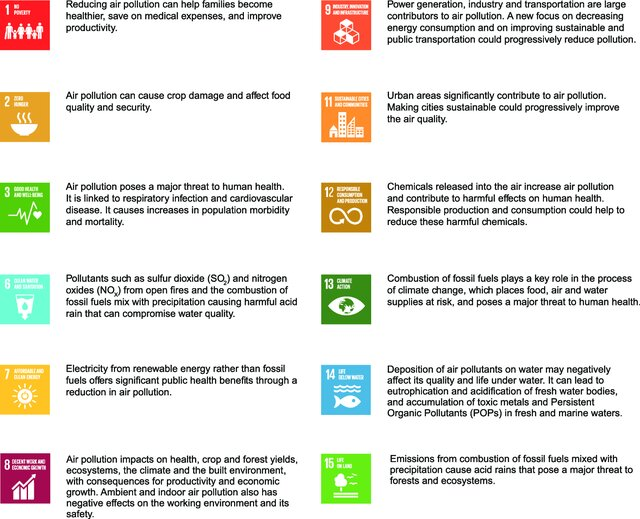
\includegraphics[width=\textwidth]{figs/chap2/How-air-pollution-relates-to-the-UN-Sustainable-Development-Goals_W640.jpg}
    \caption{How air pollution relates to the SDGs \citep{aq2017eu}}
    \label{fig:chap2_fig3}
\end{figure}
\begin{figure}[tbh!]
    \centering
    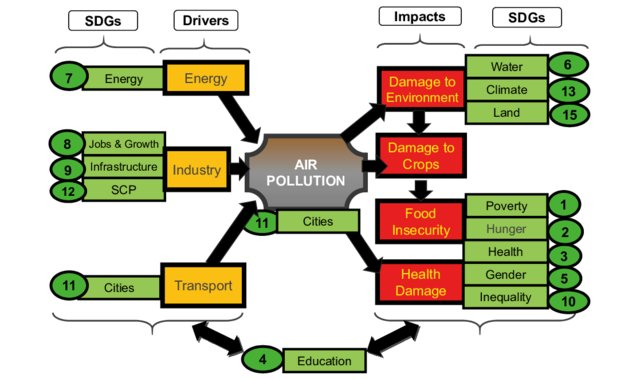
\includegraphics[width=\textwidth]{figs/chap2/Relation-of-SDGs-to-Air-Pollutions-Drivers-and-Impacts.jpg}
    \caption{Relation of SDGs to air pollution drivers and impacts \citep{elder2016strengthening}}
    \label{fig:chap2_fig4}
\end{figure}
In Figures \ref{fig:chap2_fig3} and \ref{fig:chap2_fig4}, I illustrate the connection between air pollution and the Sustainable Development Goals (SDGs) using insights from the earlier study by \citep{aq2017eu}. Additionally, I depict the relation between SDGs and the drivers and impacts of air pollution, as highlighted in the work by \citep{elder2016strengthening}. 
\begin{itemize}
    \item Goal 1 - No Poverty: Individuals and families experiencing poverty are more susceptible to the adverse effects of air pollution, particularly those reliant on outdoor labor, such as sulphur mining in active volcanoes.
    \item  Goal 2 - Zero Hunger: Air pollution has the potential to diminish crop yields and agricultural productivity, as evidenced by studies like \citep{avnery2011global}.
    \item Goal 3 - Health and Well-being: Air pollution poses a significant threat to human health \citep{who2020world}, leading to heightened morbidity and mortality rates.
    \item Goal 4 - Education: There is an expectation that educating the population will contribute to the reduction of air pollution and its future impacts.
    \item Goal 5 - Gender equality: In certain countries, women, especially those exposed to indoor air pollution from cook stoves, are more likely to bear the brunt of air pollution.
    \item Goal 6 - Water and sanitation: Pollutants like SO\textsubscript{2} and NO\textsubscript{2}, originating from open fires and fossil fuel combustion, can mix with precipitation, resulting in harmful acid rain that compromises water quality.
    \item Goal 7 - Energy: The anticipated adoption of renewable energy is expected to significantly mitigate air pollution.
    \item Goal 8 - Economic growth: Air pollution affects health, agricultural production, and ecosystems, with repercussions for productivity and economic growth. Improving resource efficiency and decoupling economic growth from environmental degradation should contribute to reducing air pollution.
    \item Goal 9 - Infrastructure, industrialization: Power generation, industry, and transportation are major contributors to air pollution. Calls for sustainable industrialization and infrastructure, with increased resource use efficiency and the adoption of clean technologies, are expected to reduce air pollution.
    \item Goal 11 - Cities: Urban areas are significant contributors to air pollution. Making cities sustainable could progressively enhance air quality.
    \item Goal 12 - Sustainable consumption and production: Sustainable production, coupled with the removal of fossil fuel subsidies, would contribute to reducing air pollution.
    \item Goal 13 - Climate action: Simultaneously reducing greenhouse gases and air pollution requires a reduction in the combustion of fossil fuels, a key contributor to climate change.
    \item Goal 14 - Oceans: Air pollution deposition on water may affect its quality and marine life, leading to eutrophication and acidification of freshwater.
    \item Goal 15 - Biodiversity, Forest: Emissions from the combustion of fossil fuels mixed with precipitation can cause acid rain, threatening forests and ecosystems.
    \item Goal 16 - Peace: Recent armed conflicts in Ukraine and Russia, and Israel and Palestine contribute to an increase in military vehicles and weapons, causing air pollution and producing toxic dust.
\end{itemize}
\subsection{Greenhouse gas and SDGs}
GHGs are atmospheric gases that trap heat and contribute to warming the Earth causing climate change which pose a significant threat to SDGs, impacting vulnerable populations in developing and less-developed countries with intensified extreme weather events such as drought and flood, resulting in inequalities and hindering progress toward many SDGs (as shown in Figure \ref{fig:chap2_fig5}). \par
Effective action to combat climate change is articulated as the goal 13 (Climate Action), emphasizing mitigation, adaptation measures and building resilience to climate-related hazards. Actions to reduce climate risk can interact with other sustainable development objectives in positive ways (synergies) and negative ways (trade-offs) \citep{lee2023climate}. \par
\begin{figure}[tbh!]
    \centering
    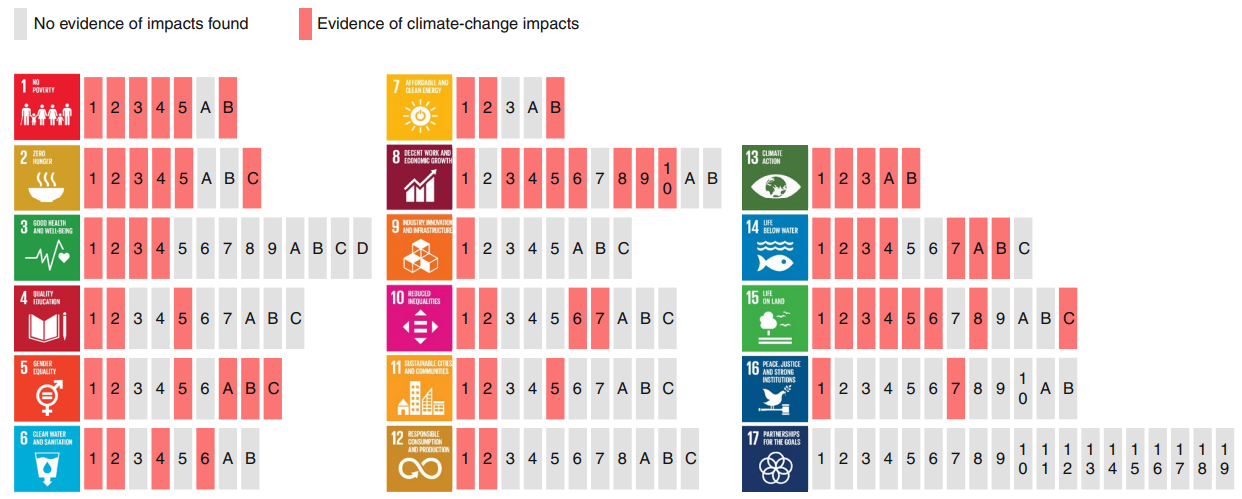
\includegraphics[width=\textwidth]{figs/chap2/impact_cc_to_sdgs.png}
    \caption{Impacts of climate change on the achievement of the SDGs \citep{fuso2019connecting}}
    \label{fig:chap2_fig5}
\end{figure}
\begin{figure}[p]
    \centering
    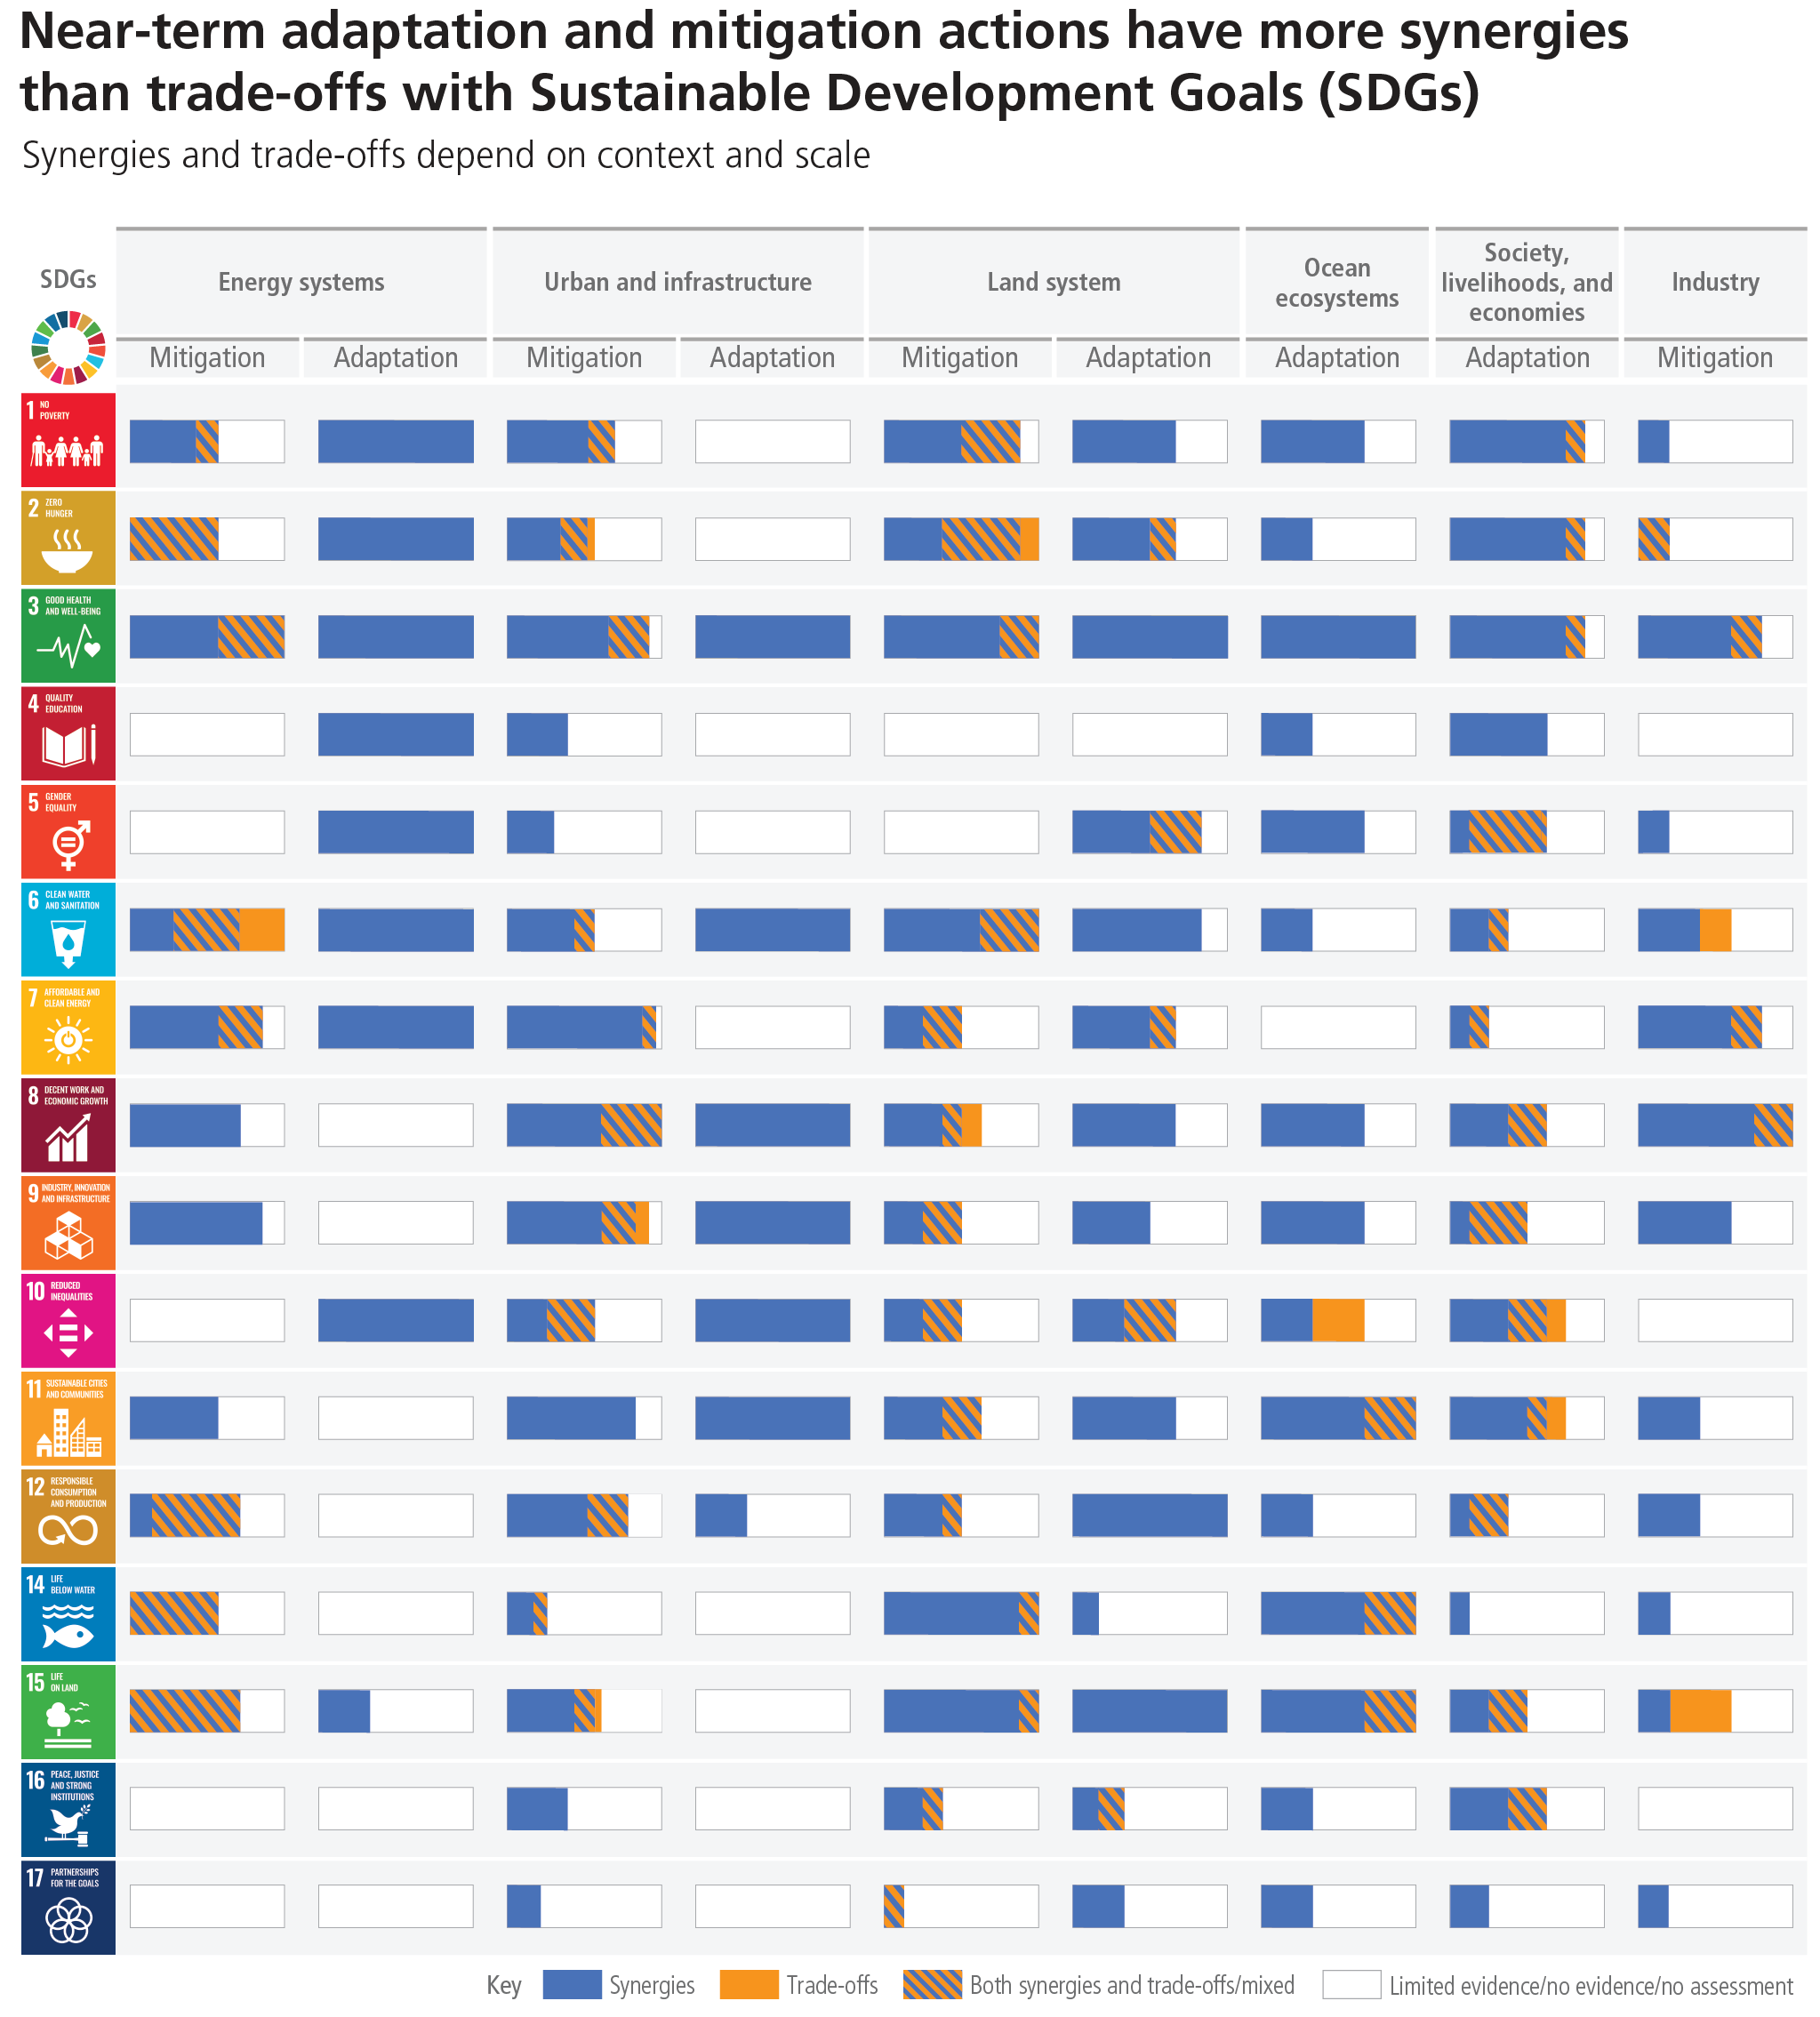
\includegraphics[width=\textwidth]{figs/chap2/IPCC_AR6_SYR_Figure_4_5.png}
    \caption[Synergies and trade-offs of climate action to other SDGs]{Synergies and trade-offs between the portfolio of climate change mitigation and adaptation options and the SDGs \citep{lee2023climate}}
    \label{fig:chap2_fig6}
\end{figure}
Figure \ref{fig:chap2_fig6} illustrate the potential synergies and trade-offs between the portfolio of climate change mitigation and adaptation options and the SDGs based on the IPCC report \citep{lee2023climate}. An example of synergy can be observed in sustainable forest management, which prevents deforestation emissions and sequesters carbon at a reasonable cost, aligning with various dimensions of sustainable development. For instance, it supports food security (SDG 2), clean water (SDG 6), and ecosystem protection (SDG 15). Another instance of synergy arises when climate adaptation measures, such as coastal or agricultural projects, empower women, leading to improvements in local incomes, health, and ecosystems \citep{ipcccfaq}. \par
Conversely, trade-offs might arise if ambitious climate change mitigation, aligned with a 1.5°C target, alters land use in ways that are detrimental to sustainable development. For instance, the conversion of natural forests, agricultural areas, or lands under indigenous or local ownership into plantations for bioenergy production could pose threats to food and water security, result in conflicts over land rights, and contribute to biodiversity loss. Additionally, trade-offs may manifest in certain regions if the transition from fossil fuels to alternative energy sources lacks careful planning, affecting existing assets, workers, and infrastructure. Effective management strategies can mitigate these trade-offs, such as enhancing bioenergy crop yields to reduce harmful land-use changes or providing retraining opportunities for workers transitioning to lower carbon sectors \citep{ipcccfaq}. \par

\subsection{Digital Earth approach and perspective}

The Digital Earth Systems approach is an approach that uses a bird's-eye view of information infrastructure to reveal the overall picture. In this context, Digital Earth has been introduced as a proposed platform for advancing the Sustainable Development Goals (SDGs) and facilitating green transformations both globally and locally, incorporating crucial SDGs variables \citep{fukui2021digital} with an illustration of the abstract architecture of a digital earth system approach is shown in Figure \ref{fig:chap2_fig7}. Essentially, we have devised various methods to effectively and accurately monitor data from diverse sources. Based on the monitored data from these sources, we formulate future policies and roadmaps, which are considered as interventions. Once an intervention is implemented, we monitor its performance and continually adjust it to align with the trajectory of sustainable development through simulations. \par
\begin{figure}[tbh!]
    \centering
    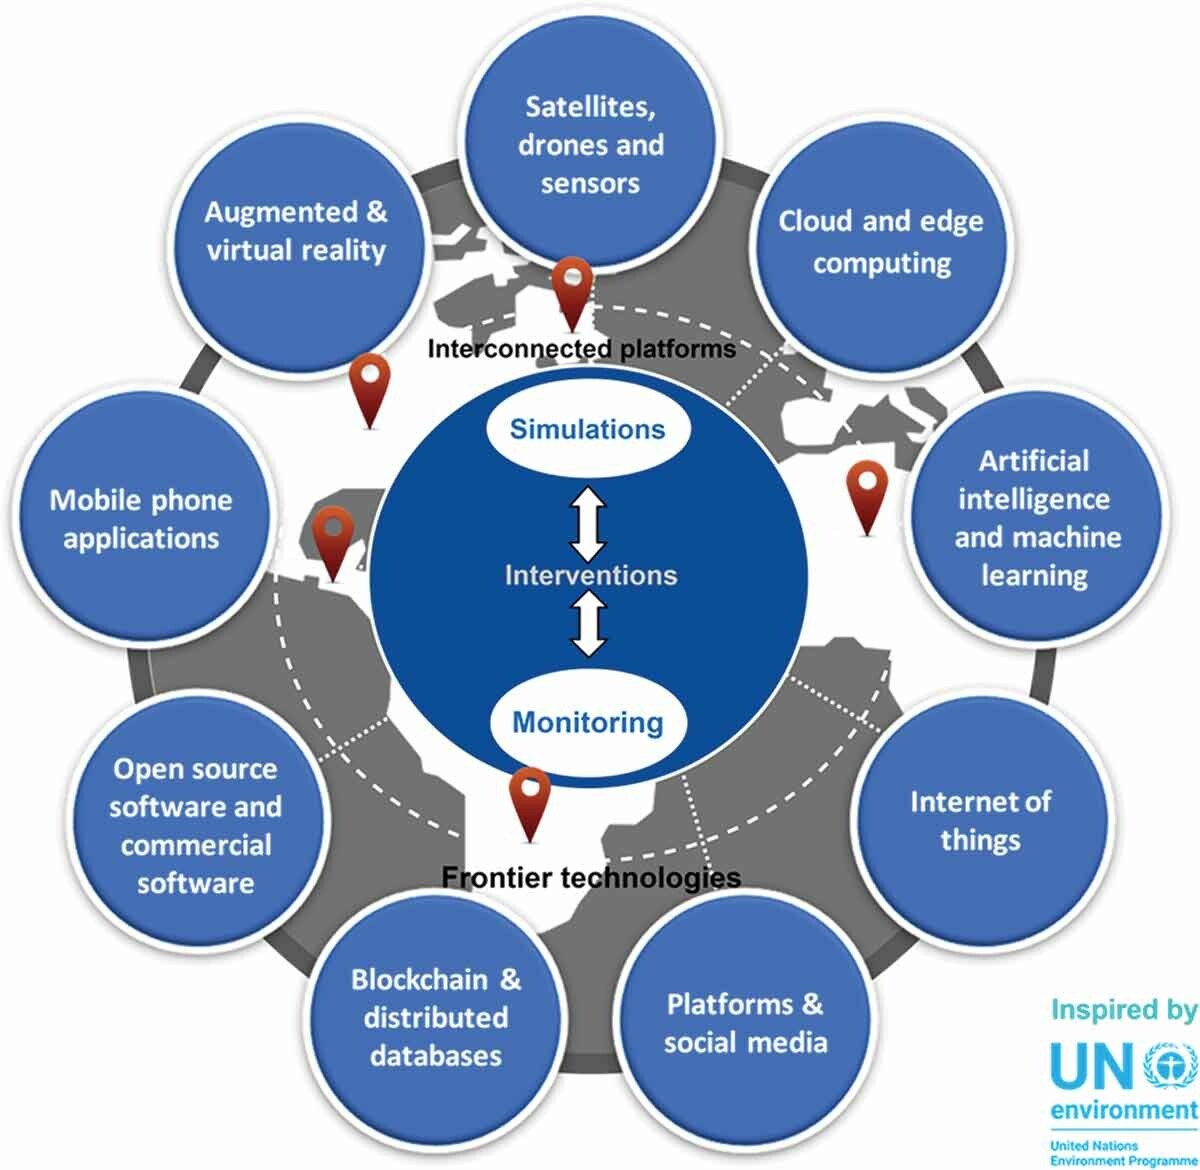
\includegraphics[width=\textwidth]{figs/chap2/digital_earth.jpg}
    \caption{An example of abstract architecture of a digital earth system \citep{fukui2021digital}}
    \label{fig:chap2_fig7}
\end{figure}

In alignment with the core concept of the digital earth system, each experiment in this study corresponds to a step in the digital earth system approach. Firstly, we employed diverse data sources, including ground-based sensor network measurements and space-based satellite observations, to analyze and quantify the primary factors contributing to changes in air pollution during intervention events. This phase can be likened to the monitoring stage in the digital earth system approach, occurring subsequent to the adoption of interventions. Based on insights from these findings, we provide evidence and recommendations for future policies. \par

In the second experiment, we also utilized multisource data to enhance the estimation of terrestrial carbon fluxes, which constitute the largest source of carbon sink on the planet. Precisely quantifying these fluxes is crucial for a thorough grasp of advancements toward carbon neutrality at both regional and global levels, thereby furnishing reliable input for the simulation phase. \par

Lastly, in the third experiment, we developed a prototype for a digital earth system dedicated to the carbon neutrality roadmap and progress tracking. This platform involved integrating multisource data for both monitoring and roadmaps purposes at the local scale. \par



